 \documentclass[conference]{IEEEtran}
\IEEEoverridecommandlockouts
% The preceding line is only needed to identify funding in the first footnote. If that is unneeded, please comment it out.
\usepackage{cite}
\usepackage{hyperref}
\usepackage[euler]{textgreek}
\usepackage{amsmath,amssymb,amsfonts}
\usepackage{algorithmic}
\usepackage{graphicx}
\usepackage{textcomp}
\usepackage{xcolor}
\usepackage{tabularx}
\usepackage{xspace}
\usepackage{subcaption}

\def\BibTeX{{\rm B\kern-.05em{\sc i\kern-.025em b}\kern-.08em
    T\kern-.1667em\lower.7ex\hbox{E}\kern-.125emX}}
\begin{document}

\title{A recommender system for scientific datasets and analysis pipelines}
\newcommand{\TG}[1]{\noindent{\color{blue}[\textsc{From Tristan:} #1]}\xspace}

\newcommand{\MM}[1]{\noindent{\color{blue}[\textsc{From Mandana:} #1]}\xspace}

\newcommand{\WIP}[1]{\noindent{\color{gray} [WIP: #1]}\xspace}

% \author{\IEEEauthorblockN{1\textsuperscript{st} Mandana Mazaheri}
% \IEEEauthorblockA{\textit{Concordia University} \\
% Montreal, Canada \\
% mndmazaheri@gmail.com}
% \and
% \IEEEauthorblockN{2\textsuperscript{nd} Tristan Glatard}
% \IEEEauthorblockA{\textit{Concordia University} \\
% Montreal, Canada \\
% tristan.glatard@concordia.ca }
% }

\author{
    \IEEEauthorblockN{Mandana Mazaheri, \color{blue}other contributors\color{black}, Tristan Glatard}
    \IEEEauthorblockA{Department of Computer Science and Software Engineering, Concordia University, Montreal, Canada}
}

\maketitle
\begin{abstract}
Scientific datasets and analysis pipelines are increasingly being shared
publicly to fulfill the requirements of open science.
However, mechanisms are lacking to reliably identify pipelines that can be
applied to a given dataset, or datasets that can be processed with a given
pipeline. Given the increasing amounts of high-quality public datasets and
pipelines, this threatens their findability and reusability. We investigate
the feasibility of a collaborative filtering system to recommend pipelines
and datasets based on provenance records generated by previous executions.
We evaluate our system using datasets and pipelines extracted from the
Canadian Open Neuroscience Platform, a national initiative for open
neuroscience. The recommendations provided by our system (AUC=0.8) are
substantially better than chance and outperform recommendations made by
domain experts using their previous knowledge as well as pipeline and dataset descriptions (AUC=0.6). In particular, domain experts often neglect
low-level technical aspects of a pipeline-dataset interaction, which are
captured by a provenance-based system. We conclude that provenance-based
pipeline and dataset recommenders are feasible and beneficial to
open-science platforms. Future work will focus on the collection of more
comprehensive provenance traces, and on deploying the system in production.


% To define a set of pipeline and datasets, we ask scientists and experts in CONP to predict the execution outcome for pairs of pipeline-dataset in which they have good or advanced level of knowledge. Then we execute all pipeline-dataset pairs which were expected to be successful and export the execution outcome to the recommender model.
% The selected approach for recommendation is collaborative filtering on explicit feedback data. We have two approaches to evaluate the results of recommender system, by cross-validations and using expert references.  \TG{summary of results}   
\end{abstract}

\begin{IEEEkeywords}
Scientific dataset, recommendation, collaborative filtering
\end{IEEEkeywords}

\section{Introduction}

Open science has emerged as a framework to improve the quality of
scientific analyses, requiring Findable, Accessible, Interoperable, and
Reusable (FAIR~\cite{wilkinson2016fair}) datasets and analysis pipelines. In
neuroscience, our main application domain of interest, platforms have
emerged to facilitate the sharing of datasets and pipelines, including
OpenNeuro~\cite{gorgolewski2017openneuro}, NeuroImaging Tools and Resources Collaboratory (NITRC~\cite{kennedy2016nitrc}), and the Canadian Open
Neuroscience Platform~\cite{Jean-Baptiste2020}. However, while public
datasets and pipelines proliferate, researchers remain unassisted in
creating relevant analyses from these resources that therefore remain
largely underutilized. Identifying the set of analysis pipelines that may
apply to a given dataset, or the list of datasets that may be processed by
a given pipeline, remains challenging. In this paper we investigate
the use of recommender systems to address this issue.

% Such platforms are critical
% ingredients of ``multiverse analyses" a type of study that evaluates the
% robustness of scientific claims in multiple analytical conditions to
% improve reproducibility~\cite{botvinik2020variability}. 

The past decades witnessed the adoption of recommender systems as the major
 technology to help customers navigate the abundant product offerings of
 online retail platforms. Two main
 recommending strategies emerged: the content-based one, which matches
 content-rich item profiles with user profiles~\cite{pazzani2007content},
 and collaborative filtering, which recommends to a given user items
 selected by users with similar preferences~\cite{rajaraman2011mining}.
 Both strategies were successfully applied and have their own strengths and
 weaknesses.
 
 We evaluate the feasibility of matching scientific pipelines and datasets
 using existing recommender system techniques. We focus on collaborative
 filtering approaches, since content-based methods would require extensive
 annotations about pipelines and datasets which are not broadly available
 despite on-going
 efforts~\cite{NeuroimagingDataModel,sansone2017dats,DATSDocumentation}.
 Collaborative filtering requires an affinity measure
 between users and items. To define such a measure between pipelines and
 datasets, we rely on past execution outcomes available through provenance
 records.

The ability of a pipeline to successfully process a dataset depends on
semantic, syntactic, and infrastructural factors. Semantic factors refer to
the content of datasets and analyses. For instance, a pipeline developed
for brain Magnetic Resonance Image (MRI) segmentation would not produce
meaningful results on other image types. Syntactic factors refer to file
formats and dataset organization. For instance, brain images are commonly
stored using the NIfTI~\cite{larobina2014medical} or
MINC~\cite{vincent2016minc} formats and pipelines developed to ingest one
format may not apply to the other one. In addition, the multiple files and
directories composing a dataset are increasingly structured using the Brain
Imaging Data Structure (BIDS~\cite{bids}) which is required by some
pipelines while other ones use their own structure. Finally,
infrastructural factors refer to the availability of functional pipelines
and datasets. For instance, some pipelines may require the loading of the
entire dataset in memory, which may not be feasible for large datasets. All
these levels must be considered in pipeline or dataset recommendations, moreover such recommendation system will bridge the gap between the semantic and other levels .

Provenance is a key concept in computational analyses, referring to the
detailed description of data transformations. Provenance records include
information mainly about the raw data used in an experiment, the analysis
software and parameters, and the execution context. In neuroimaging, the Neuro Imaging Data Model (NIDM~\cite{maumet2016sharing}) project proposed domain-specific
formats and tools based on standards from the W3C PROV working
group~\cite{missier2013w3c}. In its current form, our
recommender system merely relies on execution outcomes ("exit codes")
extracted from provenance records.

To summarize, this paper makes the following contributions:
\begin{itemize}
\item It describes a provenance-based recommender system for scientific
pipelines and datasets;
\item It evaluates the system for datasets and pipelines from the Canadian
Open Neuroscience Platform;
\item It evaluates the system against domain expert recommendations.
\end{itemize}

\TG{if not done already, explain that in neuroimaging multiple analyses can be applied to 
a given dataset and that there's multiple pipelines that implement the same analysis.}

\section{Related Work}
    
Systems have been used to recommend software in various contexts such as workflow composition and algorithm selection. However, as explained below, our context is slightly different. In neuroimaging, existing platforms focus on finding and reusing pipelines and datasets but do not include any recommender engine for pipelines and datasets.
    
\subsection{Workflow composition}

A few recommender systems were described to assist users with workflow composition, that is, to identify candidate software components to add to a given workflow. For example, the Galaxy tool recommender~\cite{kumar2021tool} recommends possible workflow components using a deep learning model trained on 18,000 bioinformatics workflows from the European Galaxy server. Recommendations depend on the definition and organization of all the tools in the workflow (so-called "higher-order workflow dependencies") instead of focusing on the last ones only. Workflow dependencies are learned using Recurrent Neural Networks, resulting in a mean accuracy of 98\%. The system is available for Galaxy users as an extension. 

Previous approaches to assisted workflow composition included loose programming, initially proposed in the PROPHETS system~\cite{lamprecht2010synthesis,naujokat2012loose,lamprecht2013user}. Loose programming enables workflow developers to program using concepts rather than accurate procedural code. Loose programming exposes to the workflow developers semantic annotations describing the functionalities of workflow components. Workflow developers can then assemble such components without having to care about correct typing, interface compatibility, platform parameters or other technical details that are taken care of through subsequent validations. PROPHETS was applied to various bioinformatics use cases, including mass spectrometry-based proteomics~\cite{palmblad2019automated}.

% \TG{how are these technical details handled?}
% However, compatibility inferred from tool annotation does not guarantee interoperability or a well-working workflow; some tools are optimized for particular datasets and may not work well, or even at all, on other data of the same type and format. It is therefore essential to validate the automatically created workflows on real input data, validating is applied by testing the workflows on real input data. 

The WINGS (Workflow INstance Generation and Specialization) system~\cite{gil2010wings} uses AI planning and semantic reasoners to assist users in creating workflows while validating that the workflows comply with the requirements of the software components and datasets. WINGS can reason about the constraints of the components and the characteristics of the data and propagate them through the workflow structure.
% \MM{in WINGS, the constraints are defined by end user then the generated workflow will be validated and passed to Pegasus to do the execution, monitoring process and resolving possible failures. NOT said HOW?!
% the (failed) execution provenance records are stored and accessible after execution :| }

These approaches assist users by matching workflow components together. Instead, in our context, the workflows (or pipelines) are already available and need to be matched to relevant datasets. Conversely, relevant analysis workflows need to be recommended for a given dataset.

\subsection{Algorithm selection}

Other recommender systems aim at selecting specific algorithms for a given problem. For instance, Oracle~\cite{oracle} selects machine-learning algorithms and models for classification and regression problems. Algorithm selection uses advanced machine learning techniques to automatically rank the best algorithms for a dataset. Model selection identifies the best hyperparameters to maximize a given prediction performance score. 

Another recent example is PennAI~\cite{la2021evaluating}, a platform that recommends suitable models given a supervised classification problem. The platform was evaluated on 165 classification problems. Results showed that matrix factorization-based recommendation systems outperform meta-learning methods.

In addition, Dyad ranking~\cite{tornede2019algorithm,tornede2020extreme} represents the algorithm and problem instance by a feature vector, and selects the best feature vectors using machine learning. The training dataset is a set of dyads ranked according to a specific preference relation. The dyad ranker learns using the neural-network-based PLNet~\cite{schafer2018dyad} algorithm. Results show that this approach outperforms many algorithm selectors while using less computation. 

All these approaches assume the existence of an objective function such as F1 score, accuracy or mean average error to compare algorithms or models that are known to apply to the problem. Instead, our goal is not to compare pipelines with each other but to predict if a given pipeline will work on a given dataset. From a methodological point of view, algorithm selection techniques are mostly content-based  while we will adopt a collaborative filtering approach.

\subsection{Finding tools and datasets in neuroimaging}

Several platforms have been developed to facilitate the sharing of tools and datasets 
in neuroimaging. For instance, NITRC~\cite{kennedy2016nitrc} provides a richly-annotated catalog of tools and datasets that can be processed in the NITRC computing environment. In OpenNeuro~\cite{markiewicz2021openneuro}, datasets complying to the BIDS data structure can be publicly shared and processed using BIDS apps.  Finally, the Neuroscience Information Framework (NIF~\cite{gardner2008neuroscience}) is a powerful search engine for neuroscience software and data. While all these platforms provide substantial services for data and tool sharing, they don't seem to include any system to assist users in the matching of pipelines and datasets. \TG{Check all the cited platforms.} Matching relevant pipelines and datasets would also enable the automated triggering of data processing when new pipelines or datasets become available. 

\section{Materials and Methods}

The goal of our recommender system is to predict if a data processing
pipeline will successfully run on a given dataset. Predictions are obtained
from provenance records created from previous pipeline executions.
Figure~\ref{fig:method} presents an overview of our system that is detailed
in the remainder of this section with our experimental methodology.

\begin{figure*}[ht]
  \centering
  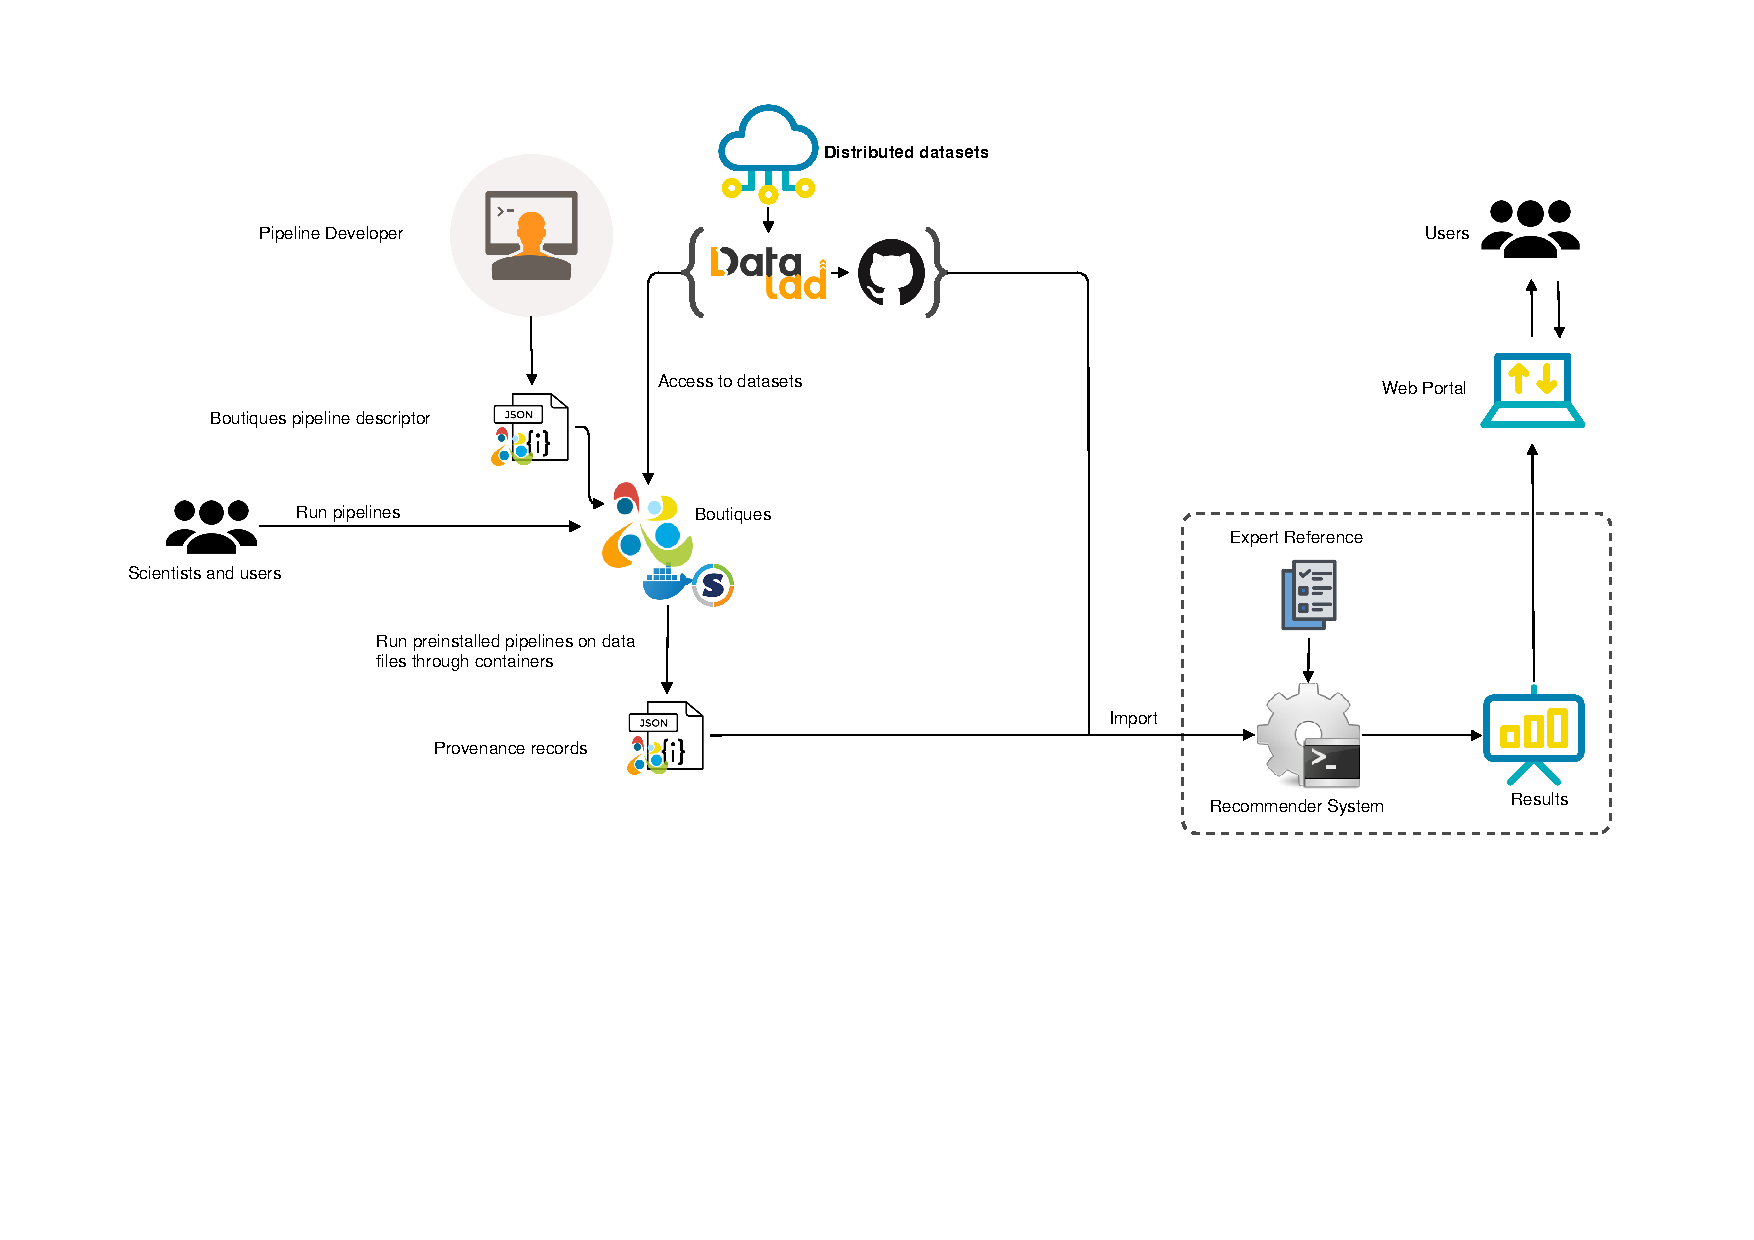
\includegraphics[width=\textwidth]{figures/Methodology.pdf}%Methodology_May17th.png}
  \caption{Overview of our recommender system }
  \label{fig:method}
  \end{figure*}  


\subsection{Data processing pipelines} 
Consistently with our motivating use case, we focused on the 64
neuroscience pipelines available in the CONP as of October
2020. Figure~\ref{fig:pipelines_tags} shows an overview of the type of data
and analyses supported by these pipelines. These pipelines are command-line
tools described by Boutiques descriptors~\cite{glatard2018boutiques} and
containerized using Docker or Singularity, which makes them portable across
a wide range of infrastructures, including local workstations, clusters,
and clouds~\cite{kiar2019serverless}. Each pipeline descriptor is stored on
the Zenodo research archive~\cite{zenodo} and identified by a permanent Digital Object
Identifier (DOI). Through the Boutiques command line, the pipelines can be
validated, installed, published, and executed. When the execution
completes, Boutiques creates a JSON provenance record containing a summary
of the execution process including the pipeline DOI, input and output file
hashes, parameter values, and exit code. Our recommendation system uses
such provenance records to track the outcome of pipeline executions on a
given dataset.
\begin{figure} 
  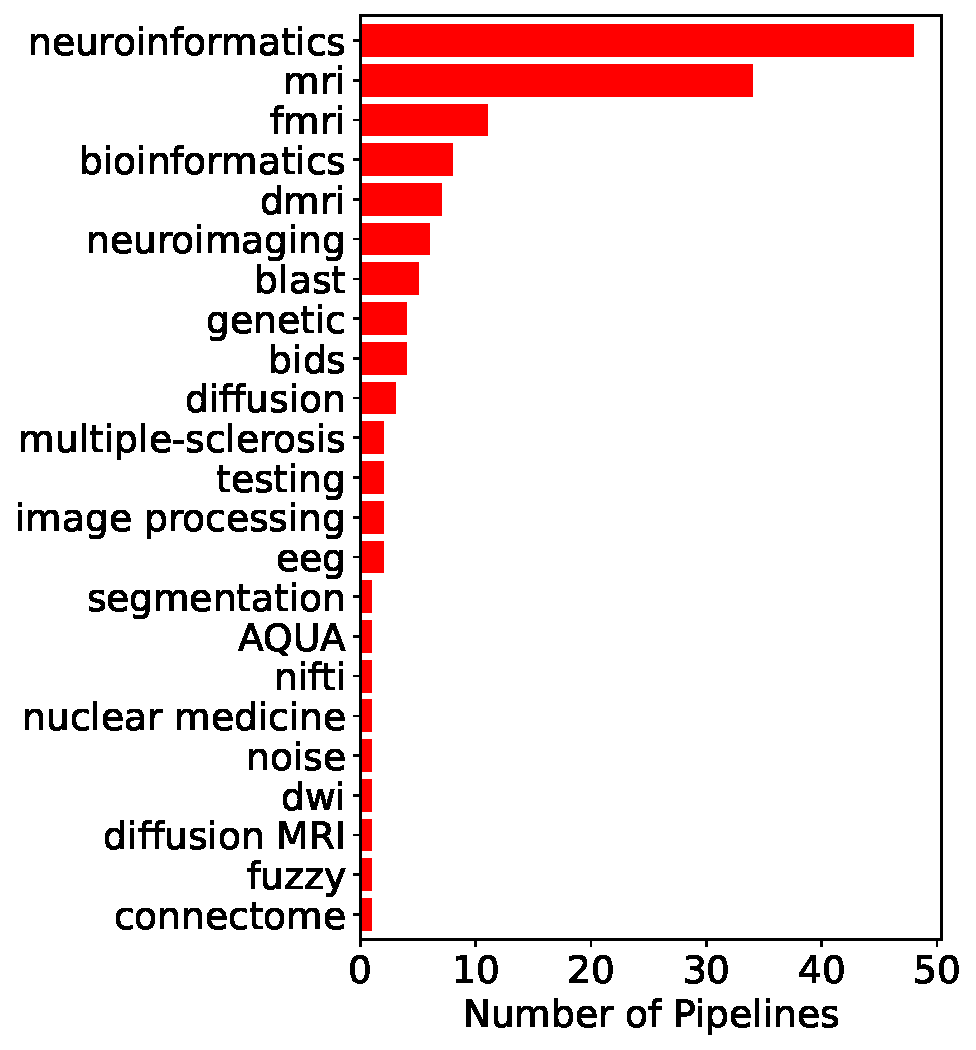
\includegraphics[width=\columnwidth]{figures/Pipelines Tag.pdf}
  \caption{Tags of available pipelines, each pipeline might have multiple tags}
  \label{fig:pipelines_tags}
\end{figure}



\subsection{Datasets} 

We used the 42 datasets available in the CONP as of October 2020,
representing a total of 2807267 files, 3078 GB, and 6330 subjects.
These datasets included neuroimaging, transcriptomics, genomics, and other
related data modalities coming from various sources distributed in Canada
and abroad (Figure~\ref{fig:datasets_modalities}). Datasets are made available through DataLad~\cite{datalad2021},
a Git-based framework that provides a uniform and version-controlled view of
distributed storage.

A DataLad dataset is a particular type of Git repository that stores
 data files using git-annex~\cite{gitannex}. Git objects contain
hashes and URLs of the data files but not the data itself. With the DataLad
client, users can download specific files and track their versions. Using
DataLad, our system matches provenance records to particular datasets
through file hashes. In addition, specific files from a given dataset can
be downloaded on demand without having to download the entire dataset. 

 In some cases, minor adjustments such as file renamings or exclusions (on 8/22 of tested datasets) to the organization of BIDS datasets were performed to make them fully comply to the standard specification . We did not apply any type conversion, to preserve realistic
 usage scenarios for our recommender system.
 These modifications are likely to be harmless in the sense that we should remove some subjects or sessions, while format conversions could raise pernicious issues. For example left-right errors related to symmetry of the human body caused by lack of correctly recorded the spatial orientation in conversion from DICOM to NIfTI~\cite{li2016first}. 
 
 \MM{Possible problems during DICOM to NIfTI conversion (page 22 of this paper)}
 
 \begin{figure}
  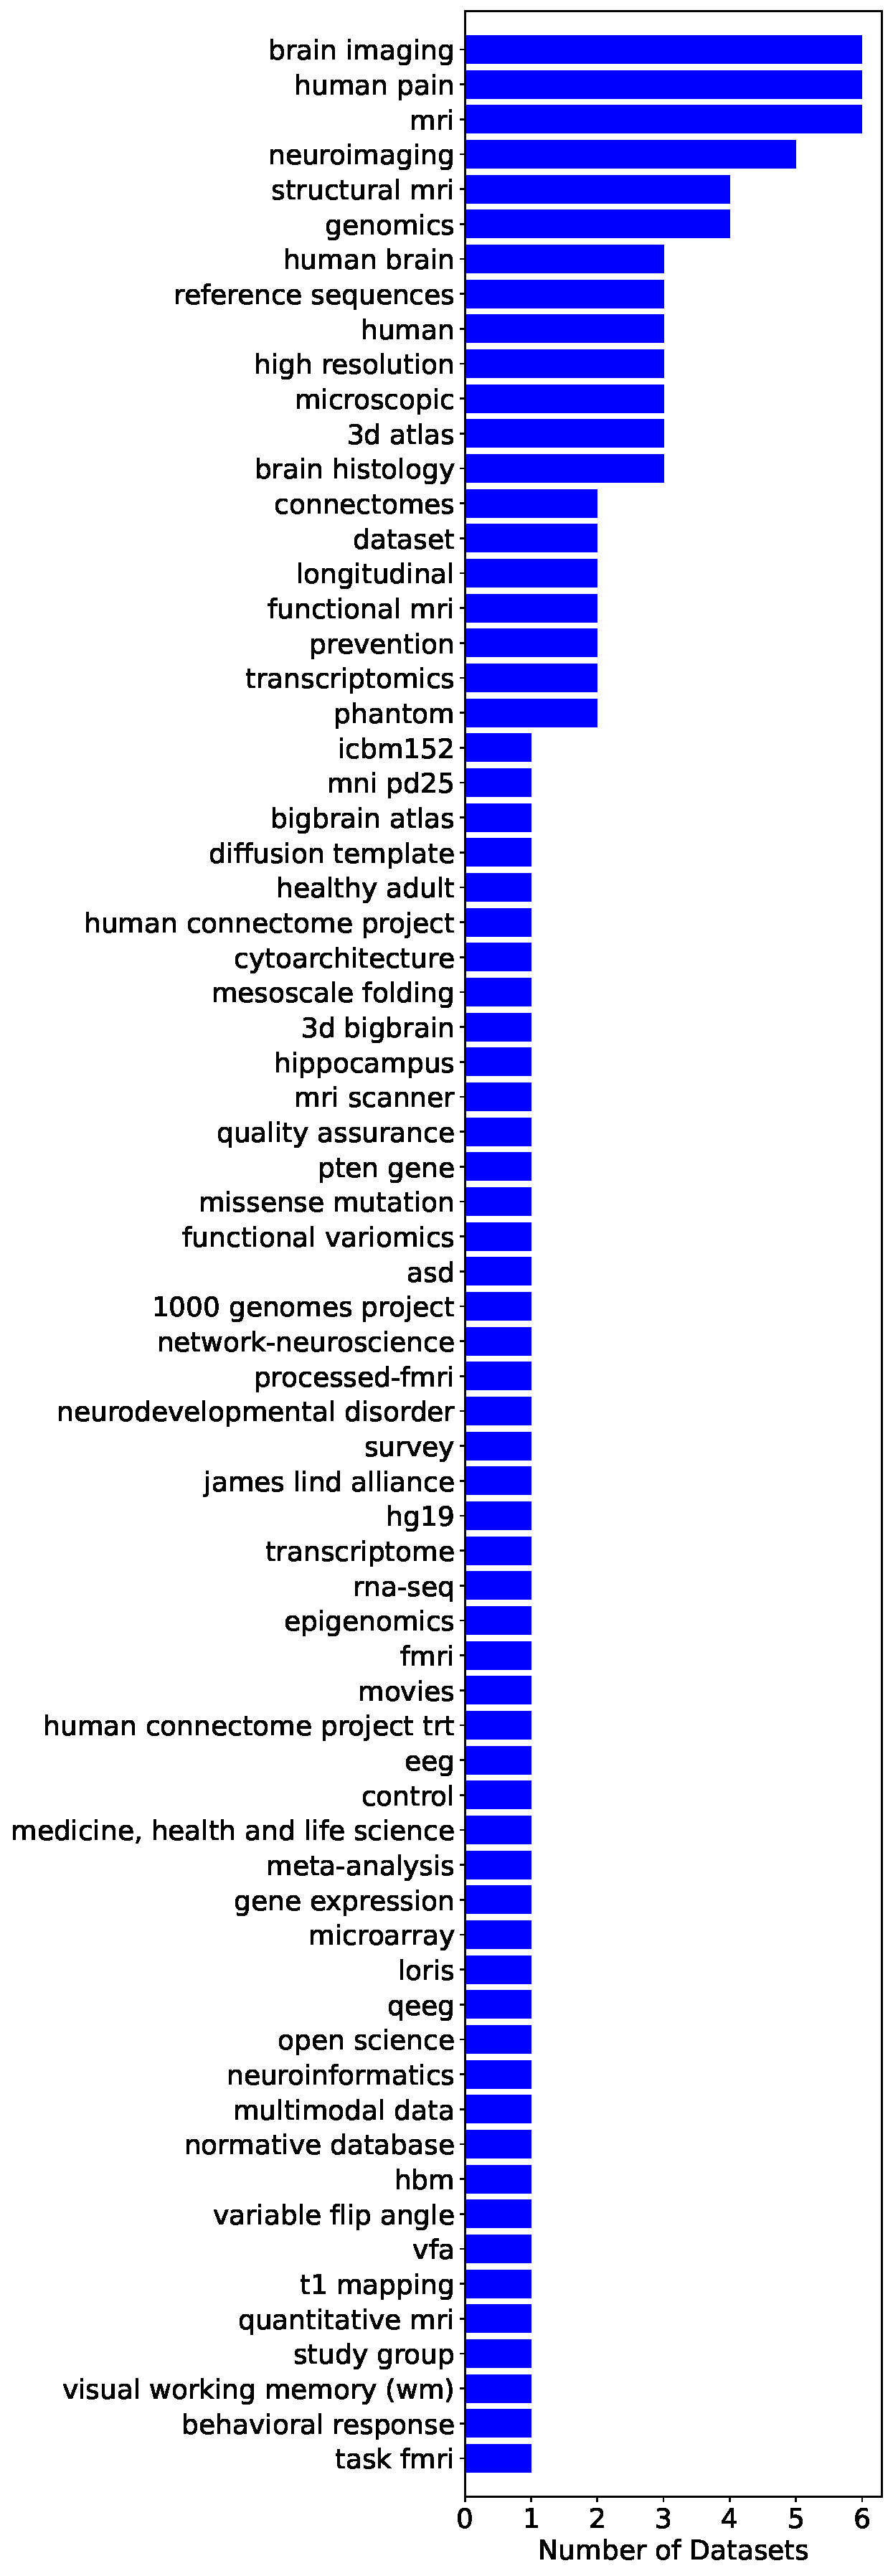
\includegraphics[width=\columnwidth]{figures/Datasets Keyword.pdf}
  \caption{Modalities of available datasets. Each dataset might have multiple keywords }
  \label{fig:datasets_modalities}
\end{figure}


\subsection{Expert Reference}

To build an expert reference, we recruited 13 experts among graduate
students, software developers and data experts at the Canadian Open
Neuroscience Platform. Since the number of pipeline-dataset pairs to
evaluate was beyond the amount that could reasonably be evaluated by a
human expert (2,688), we split our survey in two steps. In the first survey
(confidence survey), experts were asked to rate their knowledge and
confidence about each pipeline and dataset on a 4-level scale: no
knowledge, some knowledge, good knowledge, expert knowledge. In the second
survey (prediction survey), experts were ask to predict the execution
outcome (success or failure) for all pipeline-dataset pairs in which they
had indicated good or expert knowledge in the first survey for both the
pipeline and the dataset. In both surveys, all the names of pipelines and datasets were clickable and with a link to their specific page on the CONP portal that the experts were able to see all the details about them, the forms for the surveys are available at \href{https://github.com/mandana-mazaheri/Pipelines-datasets-recommender-paper/blob/master/data}{this github repository}. The data for these surveys was collected between November 2020 and March 2021.


\subsection{Provenance records} 

Similar to pipeline descriptors, Boutiques provenance records can be
published to Zenodo, which makes them publicly and permanently accessible.
We created provenance records for each pipeline-dataset pair for which at least one expert predicted successful execution. To generate a provenance record we execute a pipeline using an invocation file including all required parameters for that pipeline. The instructions for generating the invocations are available through boutiques for each pipeline. We mostly use default parameters and create minimal invocations, however, to execute some pipelines we needed editorial choices or domain experts' assistance to generate a working invocation file. Once a valid invocation is generated for a pipeline, we can use the invocation and execute the pipeline through boutiques command line.
The provenance records were entered in a database together with the file hashes of all datasets retrieved using DataLad. From this database, we generated (pipeline,
dataset, execution outcome) triplets to use in our recommender system.


% ------
% in order to match file hashes in the provenance records with actual dataset 

% The goal is to figure out that on which dataset a candidate pipeline has been executed by investigating the provenance record generated while executing the pipeline. For each executed pipeline, the provenance record contains pipeline information and input files' names and hashes. The name of the dataset is extracted by matching the file hashes in the provenance record with file hashes in datalad datasets. Finally, for each pair of pipeline and datalad dataset, we will have the status of the running process by looking at the 'exit-code' field in the provenance record. 

\subsection{Recommender system}

Collaborative filtering predicts the rating of a given item (dataset in our
case) by a given user (pipeline in our case) from the ``utility
matrix" containing previous ratings~\cite{rajaraman2011mining}.
%in which the items recommended to a user are those preferred by similar
%users. 
Two  approaches are commonly used: neighbor-based
methods~\cite{koren2015advances} and latent factor
models~\cite{koren2009matrix,bokde2015matrix}. Neighbor-based collaborative
filtering, also known as k nearest neighbors, identifies
like-minded users or similar items based on the similarity of entries in
the utility matrix. In contrast, latent factor models, the method that we used, represent items and
users in a latent space obtained from a factorization of the
utility matrix $r$ in a user matrix $p$ and an item matrix $q$. The
factorization is learned by minimizing the least square error between the
available ratings and the ratings predicted by the factorization:
\begin{equation} \tag{1}
   \min_{q_{*},p_{*}} \sum_{(u,i) \epsilon \kappa }  (r_{ui}-q_{i}^{T}p_{u})^{^2}+\lambda \left ( \left \| q_{i}\right \|^2+\left \| p_{u}\right \|^2 \right )            \label{eq}
\end{equation}
where $\kappa$ is the set of user-item pairs for which $r_{ui}$, the rating of item
$i$ by user $u$, is available. Unknown elements of the utility matrix are
predicted by the dot product of the corresponding vectors in $q$ and $p$.
In our case, pipelines represent users, datasets represent items, execution
outcomes represent ratings, and $\kappa$ is the set of pipeline-dataset
pairs for which provenance records are available. Two minimization methods are
commonly used: stochastic gradient descent and alternating least squares
(ALS). We used ALS as implemented in the
Spark Machine Learning library (spark.ml). 

All the 

% -------------------------------------
% The latent features will be calculated by optimizing the following equation \cite{hu2008collaborative} :
% \begin{equation} \tag{1}
%   min_{x_{*},y_{*}} \sum_{u,i} c_{ui}(p_{ui}-x_{u}^{T}y_{i})^{^2}+\lambda \left ( \sum _{u}\left \| x_{u}\right \|^2+\sum _{i}\left \| y_{i}\right \|^2 \right )            
% \end{equation}
% In this method, p\textsubscript{ui} represents the preference value which is set as equation 2, and r\textsubscript{ui} is the rating value, which points to the values in our utility matrix. 

% \begin{equation}\tag{2}
%     p_{ui} = \left\{\begin{matrix}
%  1 & r_{ui} > 0 \\ 
%  0 &  r_{ui} = 0
% \end{matrix}\right.
% \end{equation}
% Also, c\textsubscript{ui} represents the confidence value in this model and is calculated as equation 3 in which \textalpha{} is a constant to control the increase in rating value since in implicit feedback data there is no upper bound for rating values. 
% \begin{equation}\tag{3}
%     c_{ui} = 1 + \alpha r_{ui}
% \end{equation}
% The result of this method would be a list of N recommended items for a specific user, of which N is specified as an input for the implemented function in this library.

%     In our project we apply iALS method to each one of the four utility matrices, then we have four lists of dataset recommendations for each pipeline and four lists of recommended pipelines for each dataset. 
% \subsection{Results aggregation} 
% When applying ALS model on the utility matris of pipeline executions we will have the latent factors and will be able to
% When applying the iALS model on each utility matrix we will be provided with a list of recommendations for each dataset and pipelines given the other. We apply majority voting on the recommendation lists which are extracted from the first three utility matrices, focusing on successful executions. However, the fourth utility matrix is filled with the number of failed executions, therefore, the recommendation list for this matrix represents the pipelines or datasets which are going to fail rather than succeed. Finally, we make sure that there is no common item between these two lists.

%By applying the confidence matrix to the experts' expectation matrix we will have a weighted matrix of expectations for all pairs of pipeline-dataset. Then, we are able to compare the aggregated result of our recommendation system with this matrix and evaluate our recommender.



% \begin{figure}[t]
% \centering%\rule{0.8\textwidth}{0.3\textwidth}
% \includegraphics[scale= 0.10]{ExpertsOriginalCommentsTrimmed.png}
% \caption{Experts' Expectation Matrix}
% \label{fig:experts_matrix}
% \end{figure}

% %\newpage
% \begin{figure}[t]
% \centering%\rule{0.8\textwidth}{0.3\textwidth}
% \includegraphics[scale= 0.10]{5_RealTrimmedData.png}
% \caption{Pipeline executions}
% \label{fig:execution_matrix}
% \end{figure}
% %\newpage

\section{Results}

We evaluated our approach in two different ways. First, 
we compared the expert predictions to 
real execution outcomes extracted from provenance records.
Second, we evaluated 
the accuracy of our recommender system through 10-fold cross validation. All of the generated provenance records are stored and accessible at~\cite{provenanceRecords}

\subsection{Expert predictions vs real executions}

% The matrix in Figure~\ref{fig:experts_matrix} shows expert predictions about successful pipeline executions on datasets. The green matrix cells represent expected successful executions 36\% , red matrix cells represent expected failures 31.5\%, and the white cells represent missing data due to the experts' lack of knowledge on the pipeline or dataset 32\%. According to the experts' expectations, we ran all the pipelines on the datasets for which at least one expert predicted to run successfully, see Figure~\ref{fig:execution_matrix}.

Figure~\ref{fig:experts_matrix} shows expert predictions of
pipeline-dataset execution outcomes. Only the 32/64 pipelines for which at
least one dataset was predicted to be successfully processed by at least
one expert are represented. Pipeline names are reported in
Table~\ref{tab:pipeline_names}. Similarly, only the 22/42 datasets for which
at least one pipeline was predicted to be successfully executed by at least
one expert are represented. Dataset names are in Table~\ref{tab:data_names}. Out of a total of 704 pipeline-dataset pairs,
the execution outcome of 37\% was predicted as failed by all the experts
(white cells), the outcome of 25\% was predicted as successful by all the
experts (dark green cells), 21\% were not known with enough confidence by
any expert (gray cells), and the outcome of the remaining ones was
predicted as successful by some experts and as failed by other experts. The
large fraction of pipeline-dataset pairs unknown to any expert reinforces
the motivation for an automated recommender system.
\begin{figure}
\centering
  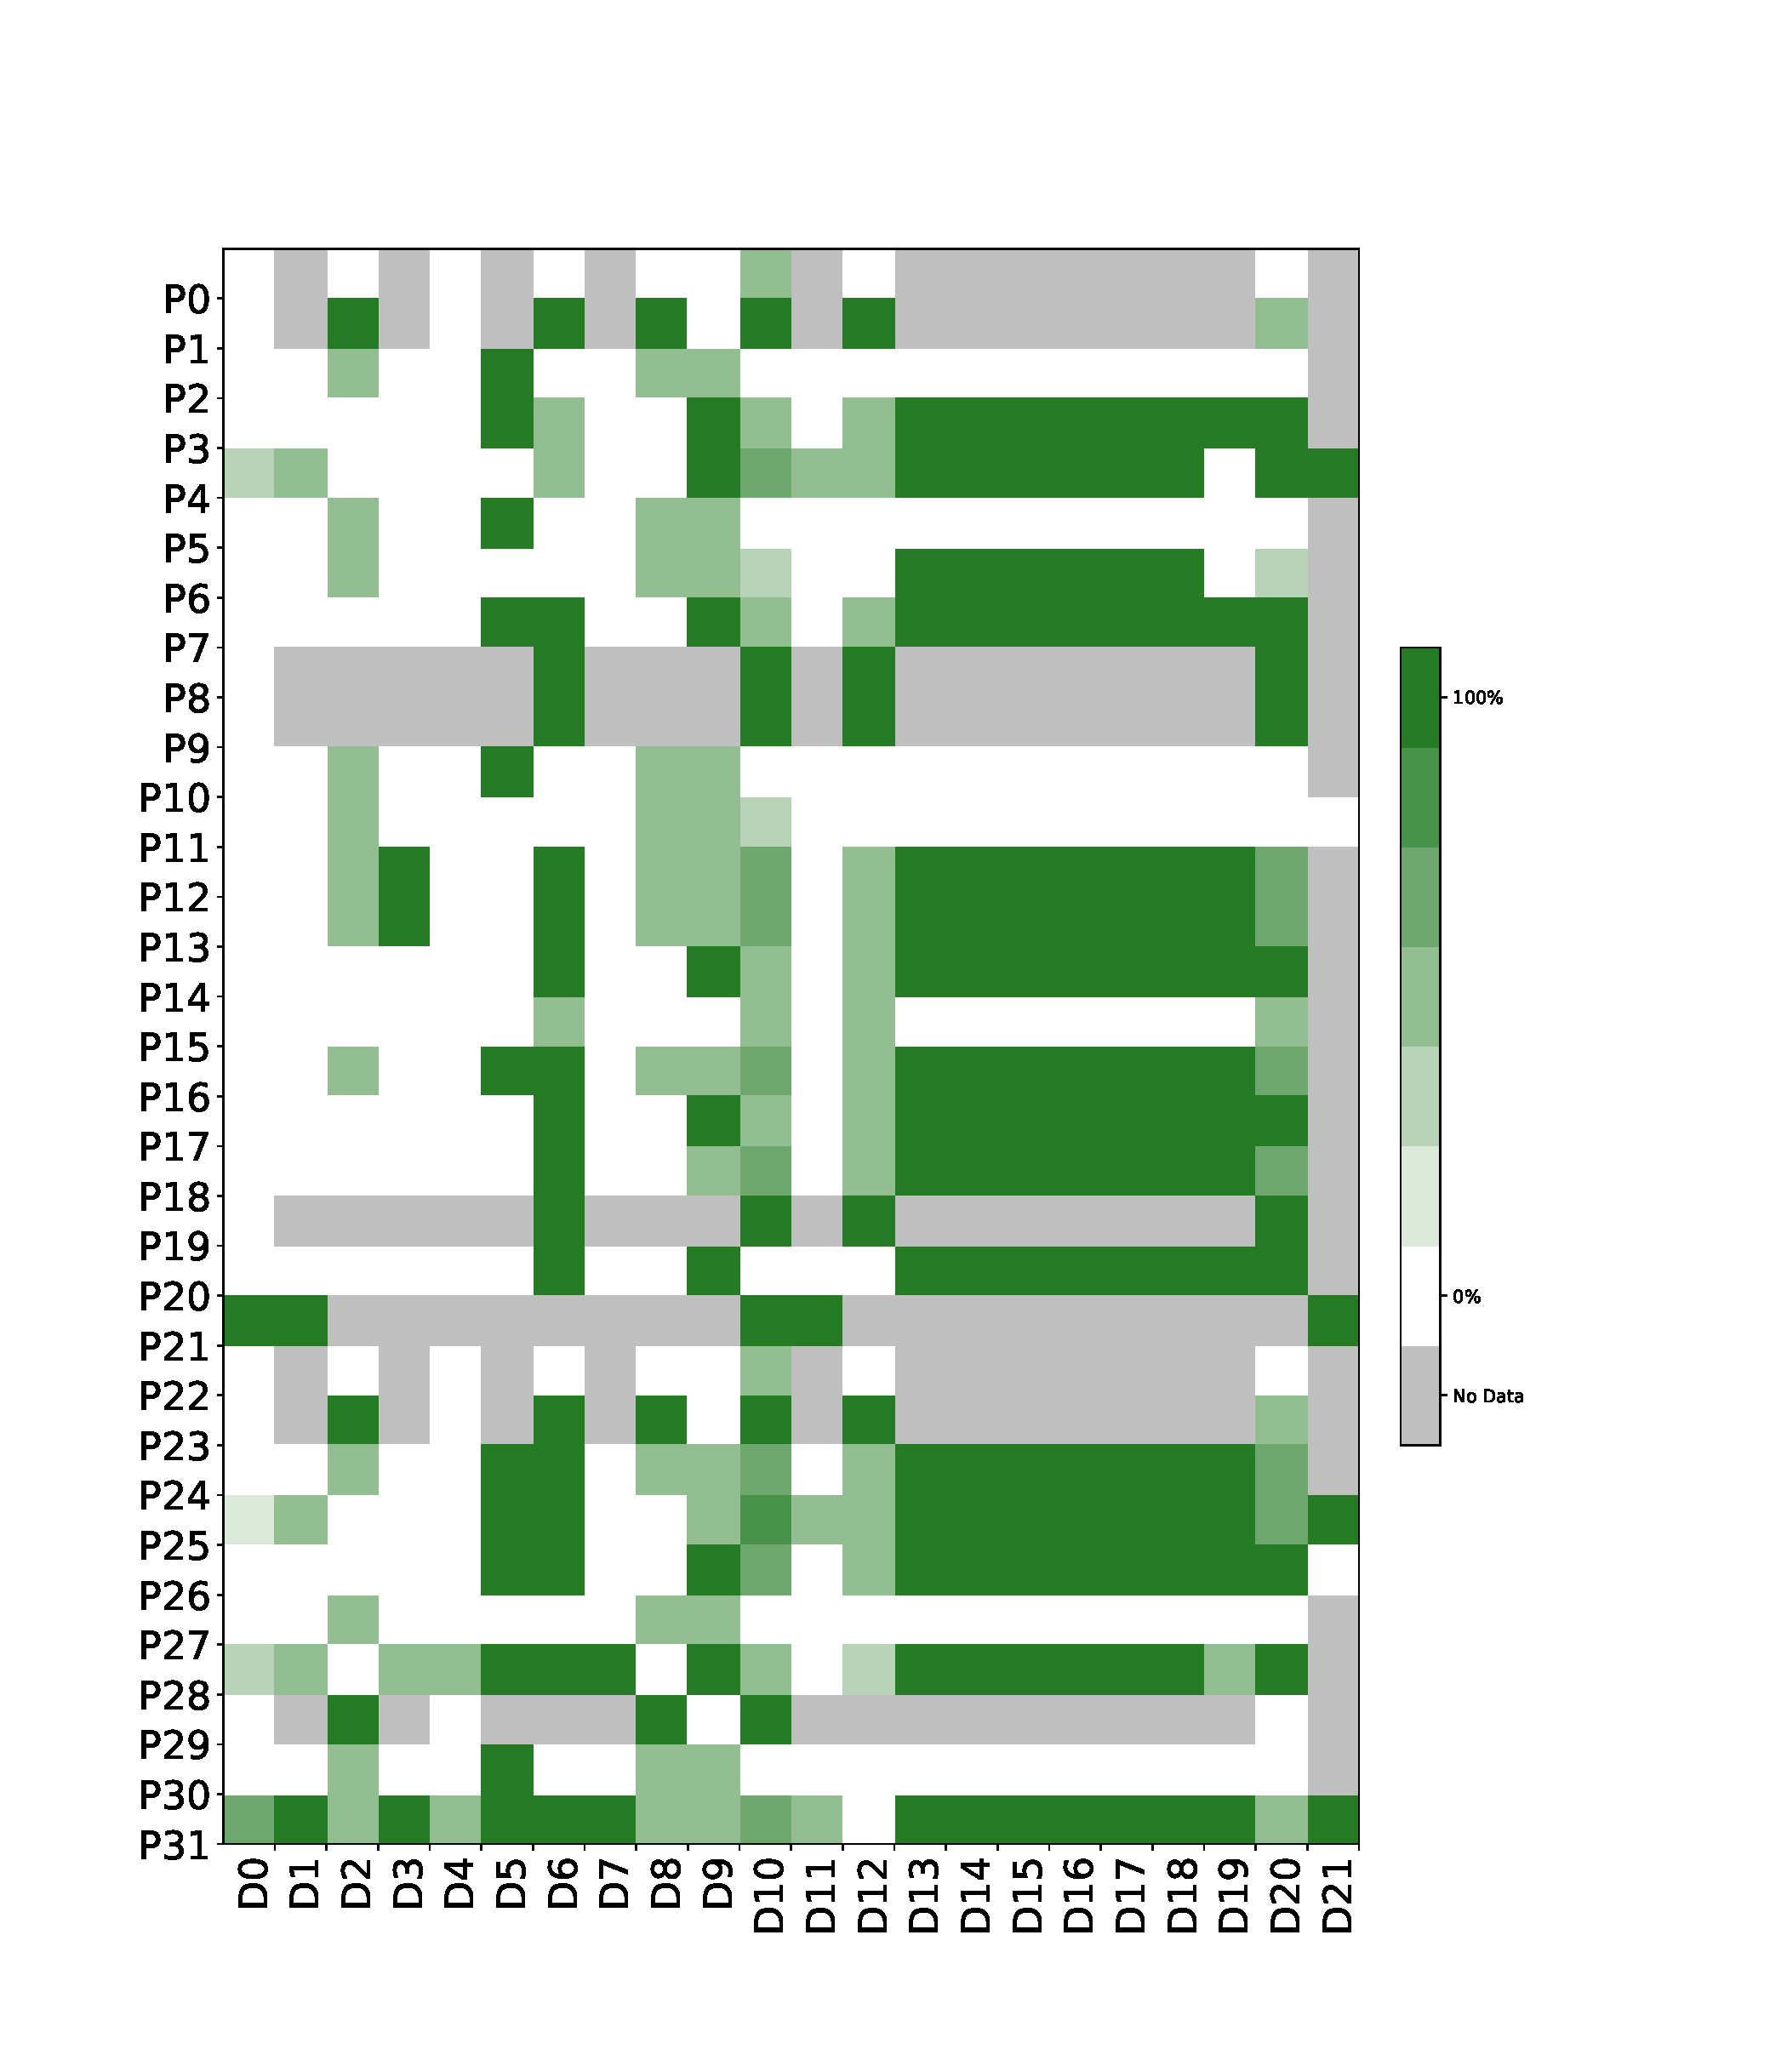
\includegraphics[width=\columnwidth]{figures/Commented Success Percentage.pdf}
  \caption{Experts confidence matrix. Shades of green represent the fraction of experts with good or advanced knowledge about the pipeline and dataset who predicted successful execution. Gray means no data. The average number of experts who were asked for prediction for pipeline-dataset pairs in this matrix is 1.39 \MM{should we keep it?! ;) LOL}}
  \label{fig:experts_matrix}
\end{figure}
% The gray cells represent pairs of pipelines and datasets that there is not any expert who knows about, ?\% of cases. 
% The rest of the cells represent the percentage of experts 
% % among all experts that know the pipeline and the dataset corresponding to that cell
% that predicted a successful execution for a pair of pipeline and dataset. The color range is dark red to green and white in the middle. To specify more, a dark red cell means 0\% of experts who know the pipeline and the dataset corresponding to that cell, predicted a successful execution; it goes whiter in the middle when the rate of successful and failure predictions get closer to 50\% and ends in green as the successful prediction rate grows up to 100\%. 

\begin{figure}%[width=1.25\columnwidth]
  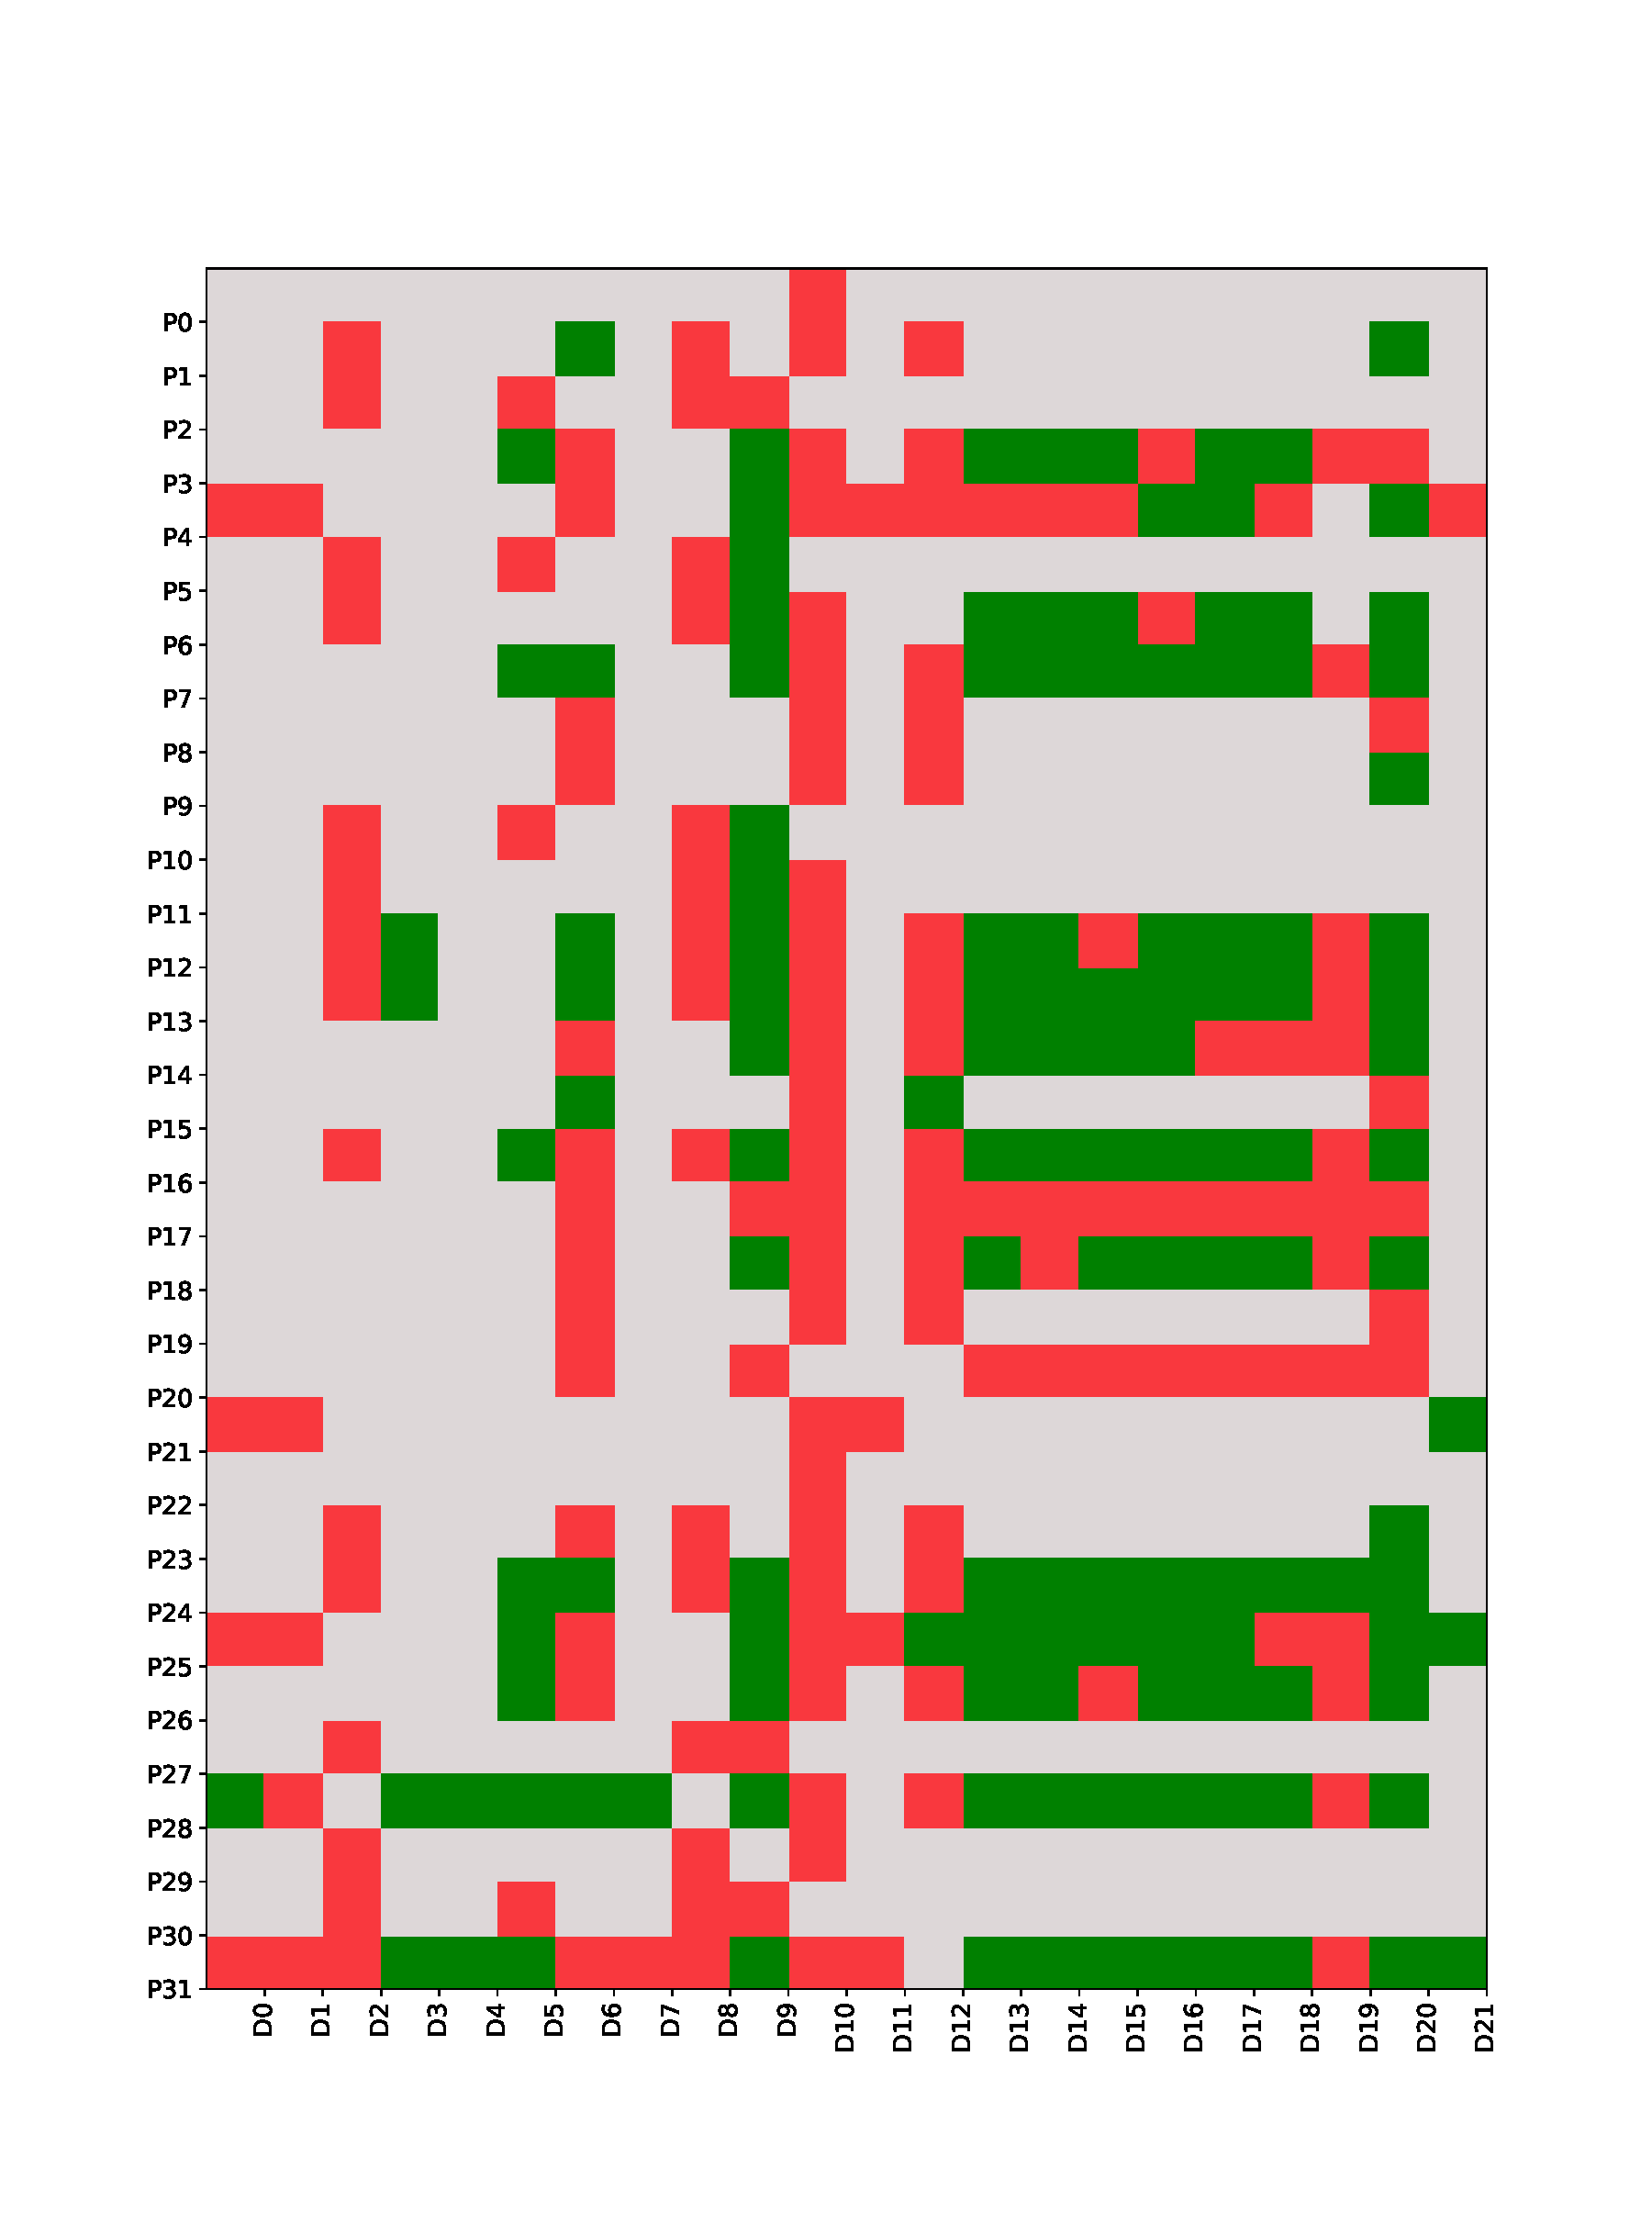
\includegraphics[width=\columnwidth]{figures/Pipeline Execution Level 2.pdf}
  \caption{Pipeline execution matrix. Green represents successful execution, red represents failures and gray represents pipeline-dataset pairs that were not executed. \TG{remove colorbar and whitespace around the matrix. Use same layout as in Fig 4.}}
  \label{fig:execution_matrix}
\end{figure}

Figure~\ref{fig:execution_matrix} shows the actual execution outcome for
all the pipeline-dataset pairs for which at least one expert predicted a
successful execution outcome (green cells in
Figure~\ref{fig:experts_matrix}). Out of 288 executed pairs, 134   were
successful and 154 failed. 
Important discrepancies are observed between expert predictions and actual
executions. Overall, 53\% of the executions that were predicted successful by
at least one expert failed in reality (red cells in
Figure~\ref{fig:execution_matrix}). In addition, the average expert
confidence was found to be significantly higher for failed executions than
for successful ones (p \textless 0.002, Figure
~\ref{fig:confidence_swarm}), which is unexpected. Expert predictions
seem to be largely unreliable. Note that we used the experts' predictions as a baseline for prediction performance comparison rather than a ground truth on the execution outcome of a given pipeline on a given dataset. 

\begin{figure}
  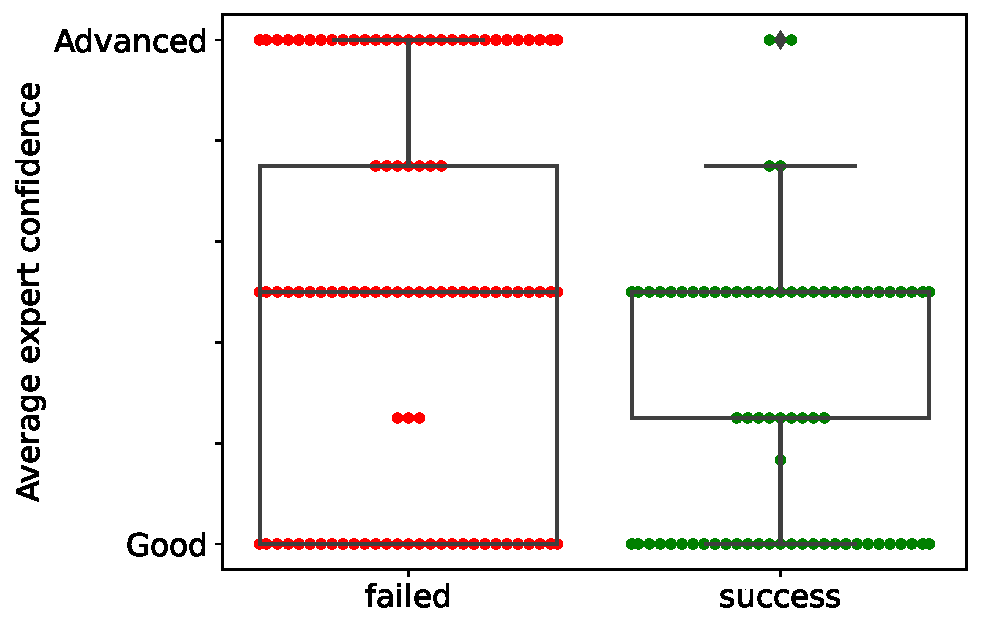
\includegraphics[width=\columnwidth]{figures/Confidence Swarm Experts.pdf}
  \caption{Expert confidence by actual execution outcome.}
  \label{fig:confidence_swarm}
\end{figure}

\begin{figure}
  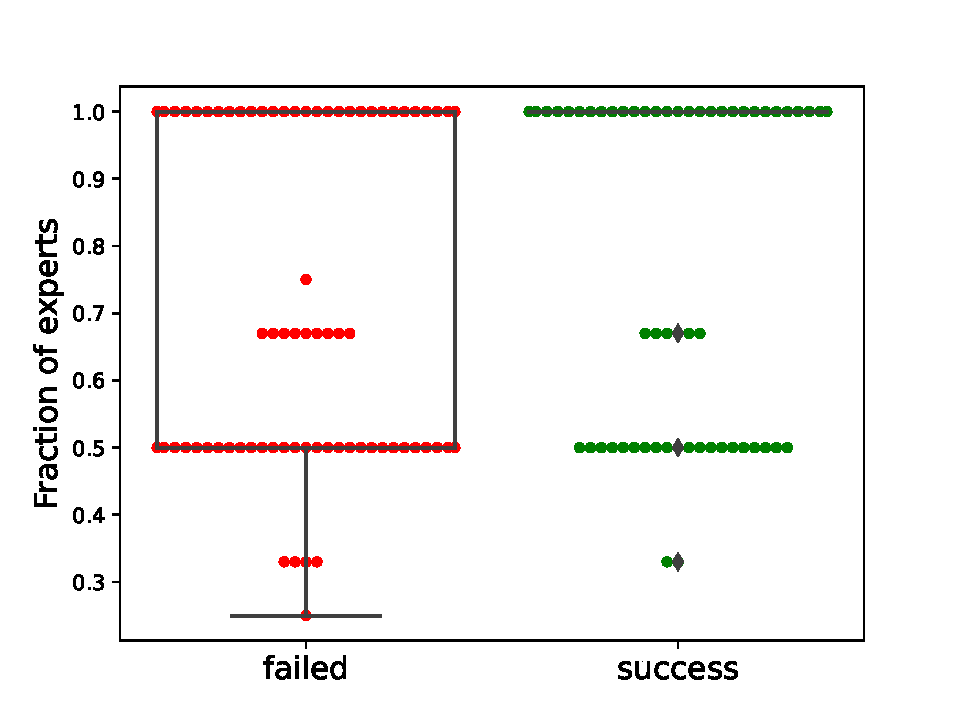
\includegraphics[width=\columnwidth]{figures/Fraction of experts.pdf}
  \caption{ Fraction of experts predicting successful executions for the executed pairs}
  \label{fig:fraction_experts}
\end{figure}


\WIP{Comment on Figure~\ref{fig:fraction_experts} }


% \begin{figure}
%   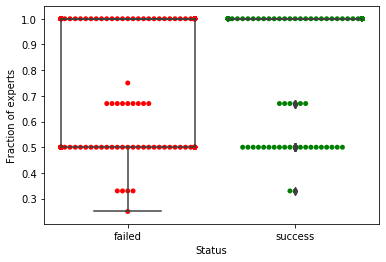
\includegraphics[scale= 0.7]{fraction_expert_success.png}%{confidence_swarm.png}
%   \caption{fraction of confident experts who predicted a successful execution for each execution case
%   t-statistic =  -4.66
% p-value =  4.66e-06 }
%   \label{fig:fraction_swarm}
% \end{figure}

Many practical reasons explain the observed discrepancy between expert
predictions and pipeline executions (Table~\ref{tab1}). First, some
datasets did not match the format required by the tested pipeline. For
instance, $P_{26}$ (fsl-first) requires anatomical images in the NIfTI file
format, however, some datasets such as $D_{12}$ (multicenter-phantom)
contain anatomical images in the MINC format.

\begin{table}[htbp]
    \caption{Execution failure causes}
    \begin{center}
        \begin{tabular}{cc}
            \hline
            \textbf{Failure reason} & \textbf{Fraction of failed executions}  \\
            \hline
            \textbf{File format not supported}    & 31\% \\
            \textbf{Type D pre-processing required}    & 18\% \\
            \textbf{Dataset not available}         & 38.5\% \\
            \textbf{Other}       & 12.5\% \\
            \hline
        \end{tabular}
        \label{tab1}
    \end{center}
\end{table}

%  Dependencies between pipelines and the
\begin{figure*}[hbt!]
\centering%\rule{0.8\textwidth}{0.3\textwidth}
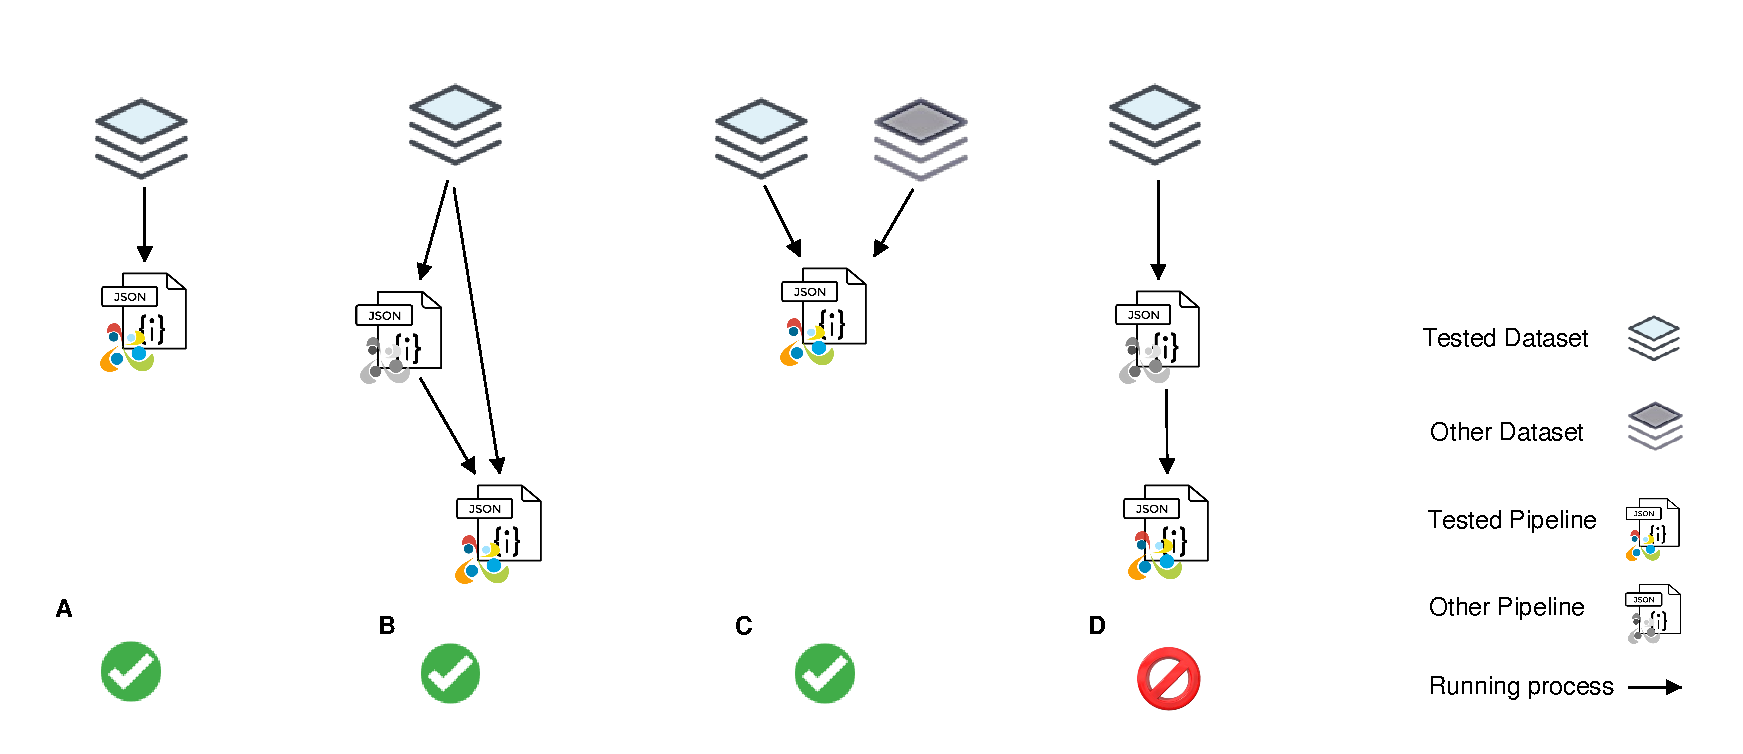
\includegraphics[width=\textwidth]{figures/Pipeline dependencies.pdf}
\caption{Types of pipeline dependencies. In Type D, the tested pipeline 
is considered not applicable to the tested dataset.}
\label{fig:pipeline_dependencies}
\end{figure*}
In addition, five pipelines ($P_{8}$, $P_{17}$, $P_{19}$, $P_{20}$ and
$P_{27}$) failed due to unresolved pre-processing requirements. We
identified four types of dependencies between pipelines
(Figure~\ref{fig:pipeline_dependencies}). Type A refers to pipelines such
as $P_{24}$ (fsl-bet) or $P_{23}$ (fsl-anat) that can be executed directly
on the tested dataset. Type B refers to pipelines that require the tested
dataset as well as the results of the application of another pipeline on
the tested dataset. For example, $P_{31}$ (oneVoxel) requires a binary mask
for its input image that is created by another pipeline. Type C refers
to pipelines that get inputs from more than one dataset. For instance, $P_7$
(ANTS Brain Extraction) and $P_9$ (ANTS Cortical Thickness) require
external templates and segmentations obtained outside of the dataset. Type
D refers to pipelines that process data derived from the tested dataset but not
the tested dataset directly.  For instance, $P_{27}$ (fsl-probtrackx2) performs
probabilistic tractography on the output of bedpostx, a pipeline that
no expert predicted to run successfully on any dataset. In a Type D
configuration, the pipeline is considered to not successfully execute on
the dataset. 
% ref: https://fsl.fmrib.ox.ac.uk/fsl/fslwiki/FDT/UserGuide)  

In addition, 4 datasets were not available for download in CONP, due to
various issues. For example, $D_{10}$ (CNeuromod) is currently not
downloadable in CONP due to on-going discussions regarding the data sharing policy.
Finally, a set of executions failed for other reasons including issues in
Boutiques pipeline descriptors or corrupted datasets.


Overall, experts seem to have neglected such practical failure reasons. In
general, experts tend to rely on their semantic understanding of the
interactions between pipelines and datasets (for instance, a given pipeline
may operate on fMRI data), while in practice, pipeline executions depend on
the lower-level syntactical and infrastructural details mentioned previously.

% They predicted \% of executions to be successful; however, only \% of executions ran successfully in practice. 


% Explaining the failures

\subsection{Recommender system evaluation} 

We evaluated the latent-factor model using 10-fold cross validation on the
pipeline execution matrix in Figure~\ref{fig:execution_matrix}. We varied
the threshold used to round predicted values to 1 (failed execution) or 2
(successful execution), resulting in the Receiver Operating Characteristic
(ROC) curve  in Figure~\ref{fig:roc-curve}. We obtained the ROC curve of
experts predictions by predicting execution outcomes using various
thresholds in the fraction of experts predicting successful execution. 

The area under curve (AUC) of our recommender system was 0.81, showing that
our model is significantly better than chance (AUC=0.5) and expert
predictions (AUC=0.63). For instance, given a rounding threshold of 1.2
(black dot in the ROC curve), out of 10 pipelines
recommended by our system for a particular dataset, 7 would be adapted to
the dataset while only 3 would not. This good performance was expected to some degree given that the pipeline execution matrix in
Figure~\ref{fig:execution_matrix} bears some sort of structure. 
A more random utility matrix would obviously be more difficult to predict.

\begin{figure}
\centering
  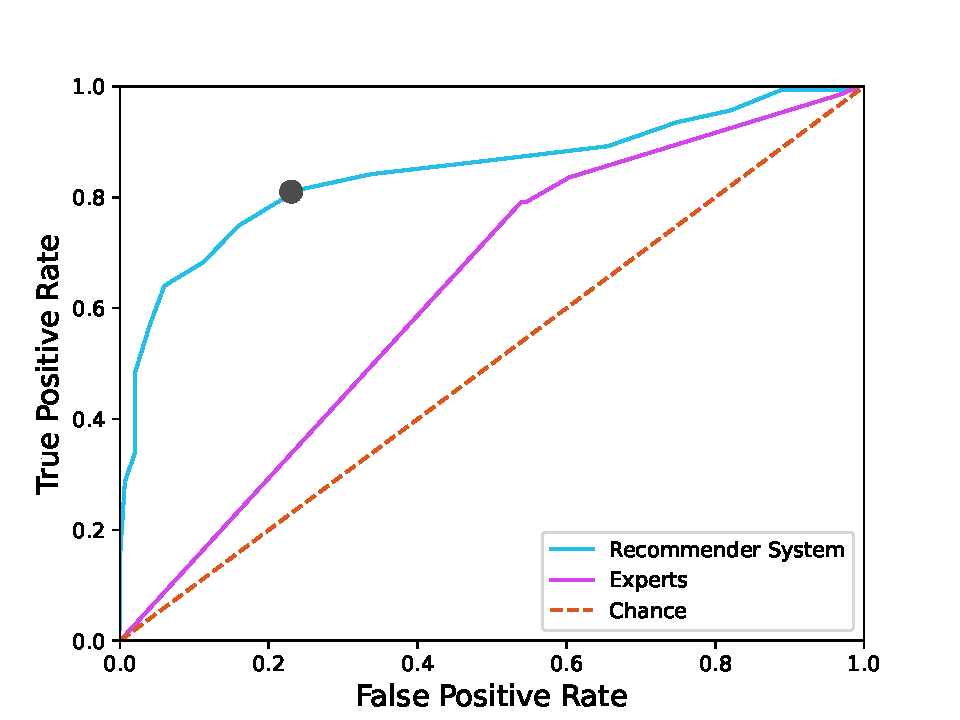
\includegraphics[width=\columnwidth]{figures/ROC Curve.pdf}
  \caption{ROC curves of experts and recommender system predictions}
  \label{fig:roc-curve}
\end{figure}

\section{Discussion}

The performance of the proposed recommender system is substantially higher
than chance and expert predictions. Predicting the successful execution
outcome of a pipeline on a given dataset is a difficult task for a human
expert as it requires a comprehensive knowledge and understanding of the
technical infrastructure, pipeline syntactical requirements, analysis
types, data formats, and data semantic types. In practice, it is common for
human experts to only master some parts of this environment. For example,
the successful processing of BIDS datasets by BIDS applications requires
datasets to pass BIDS validation, which can hardly be guessed from a
high-level overview of the dataset. In addition, pipelines or data
transfers may fail for technical reasons unknown to the experts. Automated
recommender systems based on provenance therefore have a strong added value
compared to human recommendations. 

Our experiments were conducted using one of the largest data and pipeline
sharing platform in neuroscience. Other platforms such as
NITRC~\cite{kennedy2016nitrc} contain larger collections of
pipelines and datasets, but they are not available through a consistent
interface such as Boutiques and DataLad used here, which would make
such experiments hardly feasible.

Our system architecture could potentially scale widely beyond the specific
context of CONP, as it only relies on file hashes and therefore does not
require data sharing agreements or extensive data storage. In addition, the
recommender system could leverage provenance records produced by multiple
platforms provided that they are shared for instance through Zenodo.
DataLad would detect possible duplication among datasets through file hashes. 
The framework is also expected to apply to other disciplines than neuroimaging, 
although changes in the technical context, such as datasets being stored in 
databases instead of files, may require adaptations.

In production conditions, the recommender system would rely on provenance
records of pipeline executions launched by users. While this would increase
the amount of data available, potentially resulting in more accurate
recommendations, it would also come with challenges. For instance, while
our framework models the execution outcome of a given pipeline-dataset pair
as a binary variable (success or failure), different execution outcomes may
be produced for a given pipeline-dataset pair, due to different
parametrizations or analysis types. Besides, analyses launched by less
experimented users may produce misleading provenance records. We anticipate
that the recommender could be configured to use implicit feedback to address 
this issue~\cite{hu2008collaborative}.

\section{Conclusion}

Collaborative filtering predicts the execution outcome of a given pipeline
on a given dataset with usable accuracy (AUC=0.8) in the context of the
Canadian Open Neuroscience Platform. The performance achieved by our system
outperforms
human expert recommendations, presumably due to syntactical and
infrastructural factors neglected by human experts. This recommender system is being integrated in CONP in which the recommended list of datasets or pipelines will be displayed on the CONP portal interface and available for the users, to see the mock-up for recommender interface on the CONP portal \href{https://github.com/mandana-mazaheri/Pipelines-datasets-recommender-paper/blob/master/result/mockup_for_recommender_on_portal.png}{ click here}. 

Future work will focus on the deployment of such a system in production conditions, which will require dealing with less reliable provenance records.

The framework could be extended by considering pipelines and datasets 
at a finer granularity. Pipelines can often be used in different ways 
depending on their parametrization. Different parametrizations could 
be identified in the provenance records and recommended accordingly 
for specific datasets.
Currently we rely on the available provenance records, but we could actively trigger executions to enrich our execution matrix and make more reliable predictions, more specifically, once we have a functional invocation we can create many provenance records by varying the parameters.


Besides, datasets often consist of multiple 
sub-parts corresponding to different subjects or data types. A recommender 
system could be designed to recommend analyses for such sub-parts, 
resulting in more specific recommendations.



% \TG{Summarize in 3-4 sentences what you did. Summarize the key findings: recommending pipelines and datasets from previous execution records is feasible. Besides, it is preferable than relying on experts knowledge, as it gives a more accurate technical prediction based on actual data. Our prototype can be reused and adapted to many different platforms.}


% Maybe later:

% Similar datasets, such as X, Y and Z, consistently lead to similar predictions by experts. For instance, pipeline A is expected to run successfully on all these datasets while pipeline B is expected to fail consistently. 

% The behavior of some pipelines are similar to each other. For example FslBet601, fslbet and fslstat have similar results for some datasets. Moreover, there are some blank rows or columns in this matrix which the reason has been empty dataset, not compatible formats or some challenges which appeared in practice and will be explained in discussion section. 









\bibliographystyle{plain}
\bibliography{bibliography}


\begin{table}
    \centering
    \begin{tabular}{cc}
        \hline
        Index & Pipeline Name  \\
        \hline 
        $P_{0}$ & ApplyTOPUP \\
        $P_{1}$ & ApplyWarp\\
        $P_{2}$ & BIDS App -- FSL Diffusion Preprocessing\\
        $P_{3}$ & BIDS App - FreeSurfer 6.0\\
        $P_{4}$ & BIDS App - fmriprep\\
        $P_{5}$ & BIDS App - ndmg\\
        $P_{6}$ & BIDS app example\\
        $P_{7}$ & ANTS Brain Extraction\\
        $P_{8}$ & ANTS Concat Transfo\\
        $P_{9}$ & ANTS Cortical Thickness\\
        $P_{10}$ & DTIFit\\
        $P_{11}$ & Dipy Tracking and Connectome Generation\\
        $P_{12}$ & FLIRT	\\
        $P_{13}$ & FNIRT	\\
        $P_{14}$ & FreeSurfer-Recon-all\\
        $P_{15}$ & FreeSurferPipelineBatch-CentOS7\\
        $P_{16}$ & FslBet601	\\
        $P_{17}$ & ICA\_AROMA	\\
        $P_{18}$ & MCFLIRT	\\
        $P_{19}$ &MRIQC	\\
        $P_{20}$ & PreFreeSurferPipelineBatch	\\
        $P_{21}$ & SPARK (stage 1 of 3)	\\
        $P_{22}$ & TOPUP	\\
        $P_{23}$ & fsl\_anat	\\
        $P_{24}$ & fsl\_bet	\\
        $P_{25}$ & fsl\_fast	\\
        $P_{26}$ & fsl\_first	\\
        $P_{27}$ & fsl\_probtrackx2	\\
        $P_{28}$ & fslstats	\\
        $P_{29}$ &mask2boundary\\
        $P_{30}$ & ndmg	\\
        $P_{31}$ & oneVoxel\\
        \hline\\
        &
    \end{tabular}
    \caption{Pipeline names}
    \label{tab:pipeline_names}
\end{table}

% \begin{figure*}[hbt!]
% \centering%\rule{0.8\textwidth}{0.3\textwidth}
% \includegraphics[scale= 0.13]{pipeline index.png}
% \caption{Pipelines' indices}
% \label{fig:pipeline_index}
% \end{figure*}

% \begin{figure*}[hbt!]
% \centering%\rule{0.8\textwidth}{0.3\textwidth}
% \includegraphics[width=\textwidth,scale= 0.5]{Dataset Index.png}
% \caption{Datasets' indices}
% \label{fig:dataset_index}
% \end{figure*}

\begin{table}
    \centering
    \begin{tabular}{cc}
        \hline
        Index & Dataset Name  \\
        \hline 
        $D_{0}$ & BigBrain \\[5pt]
        $D_{1}$ & BigBrain\_3DClassifiedVolumes\\[5pt]
        $D_{2}$ & \parbox{3cm}{Comparing\_Perturbation\_Modes\\
        \_for\_Evaluating\_Instabilities\\
        \_in\_Neuroimaging\_\_Processed\_NKI\\
        \_RS\_Subset\_\_08\_2019\_}\\[5pt]
                &\\
        $D_{3}$ & Khanlab/BigBrainHippoUnfold\\ [5pt]      
        $D_{4}$ & Khanlab/BigBrainMRICoreg\\[5pt]
        $D_{5}$ & Khanlab/HCPUR100-Template\\[5pt]
        $D_{6}$ & \parbox{3cm}{Learning\_Naturalistic\_Structure\\
        \_Processed\_fMRI\_dataset}\\[5pt]
                 &\\
        $D_{7}$ & \parbox{3cm}{MRI\_and\_unbiased\_averages\\
        \_of\_wild\_muskrats\_\\
        \_Ondatra\_zibethicus\_\\
        \_and\_red\_squirrels\_\\
        \_Tamiasciurus\_hudsonicus\_} \\[5pt]
                 &\\        
                 
        $D_{8}$ & \parbox{3cm}{Numerically\_Perturbed\_Structural\\
                \_Connectomes\_from\_100\_individuals\_ \\in\_the\_NKI\_Rockland\_Dataset}\\[5pt]
                &\\
        $D_{9}$ & SIMON-dataset\\
        $D_{10}$ & cneuromod\\
        $D_{11}$ & mm\_neo\_atlas\\
        $D_{12}$ & multicenter-phantom\\
        $D_{13}$ & openpain/BrainNetworkChange\_Mano\\
        $D_{14}$ & openpain/cbp\_resting\\
        $D_{15}$ & openpain/placebo\_1\\
        $D_{16}$ & openpain/placebo\_predict\_tetreault\\
        $D_{17}$ & openpain/subacute\_longitudinal\_study\\
        $D_{18}$ & openpain/thermal\\
        $D_{19}$ & preventad-open\\
        $D_{20}$ & preventad-open-bids\\
        $D_{21}$ & visual-working-memory\\
        
        
        \hline \\
        &
    \end{tabular}
    \caption{Dataset names}
    \label{tab:data_names}
\end{table}

\end{document}